The main observable to distinguish the signal of nuclear recoils from
the various types of background, is the energy density $\delta$ of the
cluster.

\subsection{Signal Preselection}
To enhance the purity of the signal sample, a pre-selection was
applied, prior to a tighter selection on $\delta$: clusters with
$l_p>6.3$\unit{cm} or $\xi<0.3$ were rejected to primarily suppress
the contribution from cosmic rays. A further loose requirement
$\delta>5$ photons/pixel was also applied to remove the residual
cosmic rays background based on their low specific
ionization. Considering that the applied thresholds are very loose for
nuclear recoils with $E<1\MeV$ energies, as shown in
Fig.~\ref{fig:range}, the preselection efficiency is assumed to be
100\%. For electron recoils it is estimated on the \fe data sample,
and is measured to be $\varepsilon_{B}^{presel}=70\%$.

With this preselection, the distribution in the 2D plane
$\delta$--$l_p$ is shown in Fig.~\ref{fig:dvsl} for \ambe source and
no-source data and for the resulting background-subtracted \ambe data.
The latter distribution shows a clear component of clusters with short
length ($l_p\lesssim1$\unit{cm}) and high density ($\delta\gtrsim
10$), expected from nuclear recoils deposits.

In addition, it shows a smaller component, also present only in the
data with \ambe source, of clusters with a moderate track length,
$1.5 \lesssim l_p \lesssim 3.0$\unit{cm}, and a lower energy density
than the one characteristic of the nuclear recoils
($9\lesssim\delta\lesssim12$). Since the density is inversely
proportional to the number of active pixels $n_p$, which is correlated
to the track length, the almost linear decrease of $\delta$ as a
function of $l_p$ points to a component with fixed energy. The
$^{241}$Am is expected to produce photons with $E=59\keV$. This
hypothesis is verified by introducing an oblique selection in the
$\delta-l_p$ plane: $\abs{\delta-y}<2$, where $y=14-p_l/50$, for the
clusters with $120<l_p<250$\unit{pixels}, defining the control region
$PR$. The obtained energy spectrum for these clusters is shown in
Fig.~\ref{fig:59keV}, which indeed shows a maximum at
$E=60.9\pm3.6\keV$, within the expected resolution. These events are
thus rejected from the nuclear recoils candidates by vetoing the $PR$
phase space.

\begin{figure}[ht]
  \begin{center}
  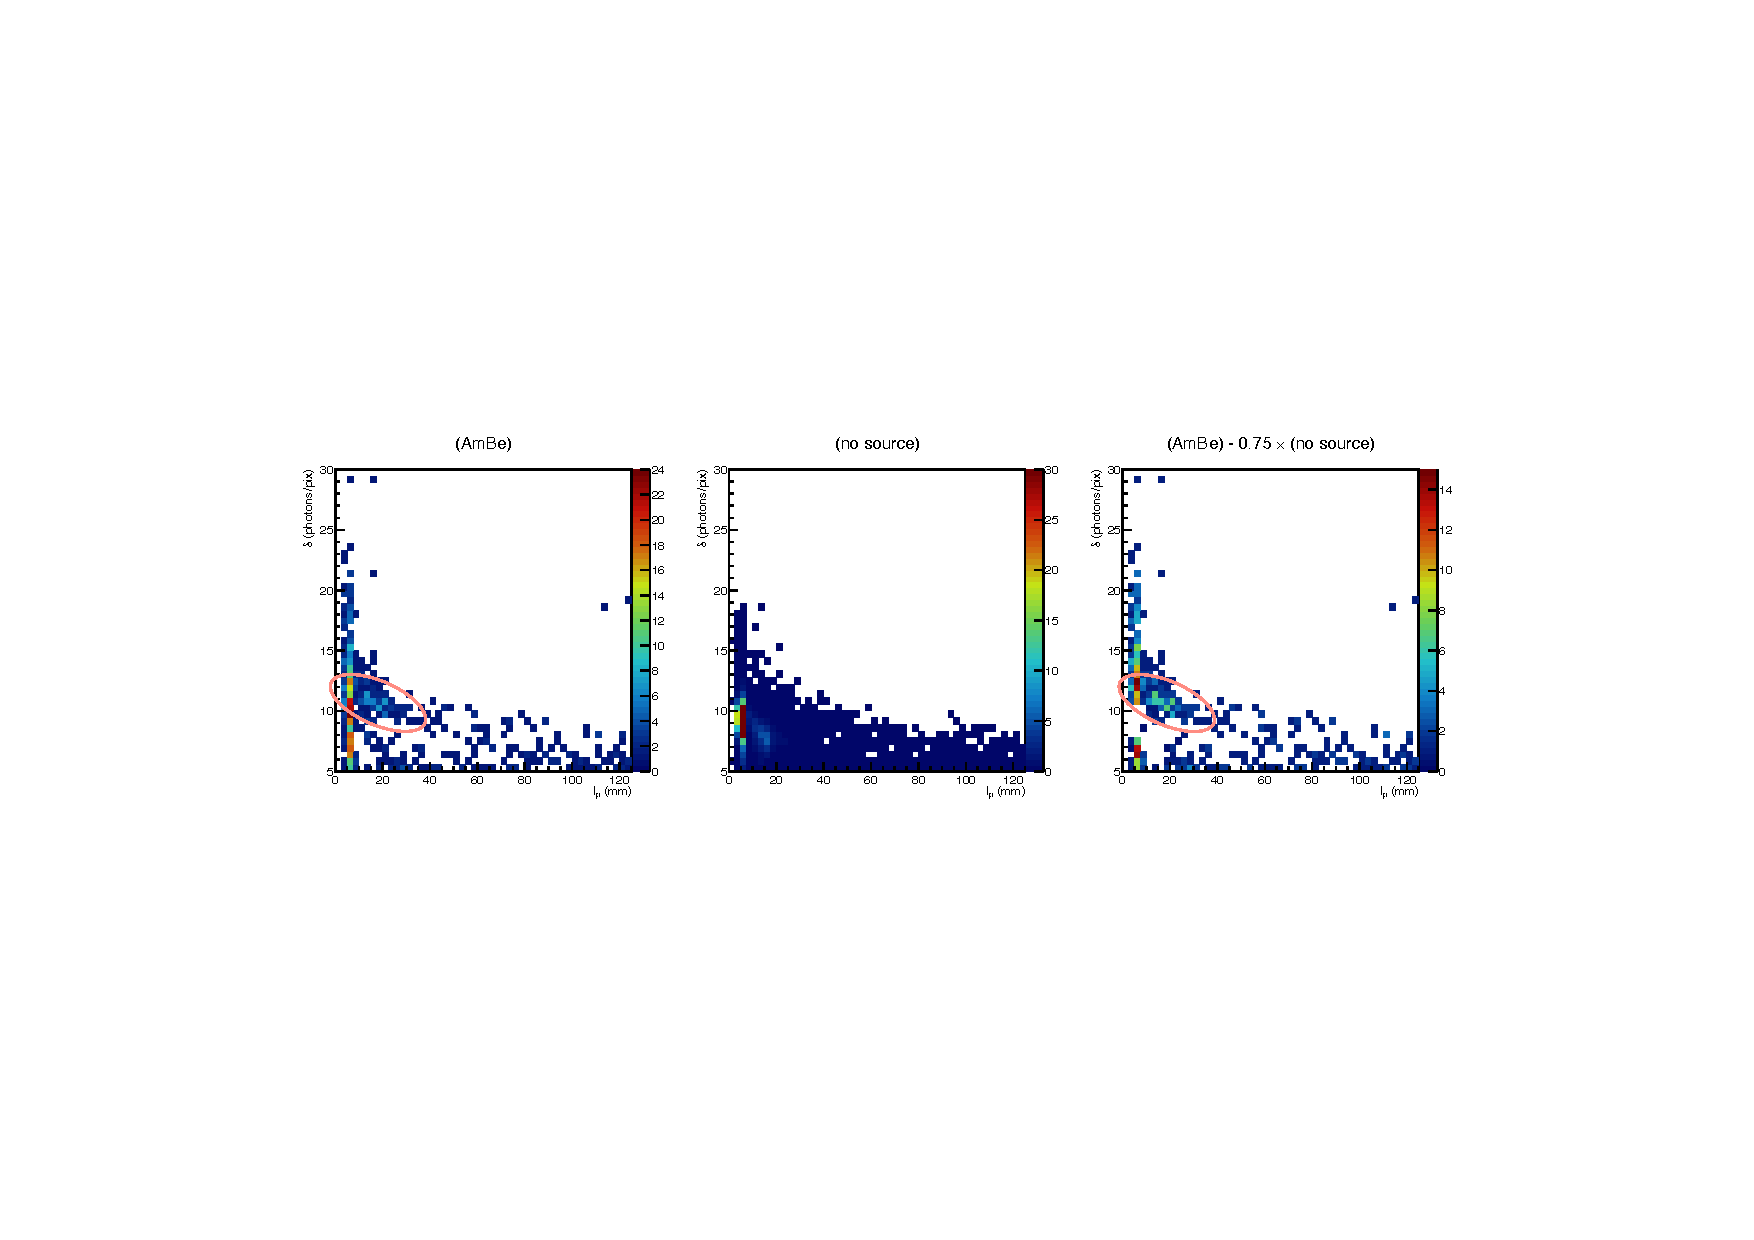
\includegraphics[width=0.90\linewidth]{figures/densityvslength_zoom}

  \caption{Supercluster light density $\delta$ versus length $l_p$,
    for data with \ambe source (left), data without any artificial source
    (middle), and the resulting background-subtracted \ambe data.  The
    normalization of data without source is to the same exposure time
    of the \ambe one, accounting for the trigger scale factor
    $\varepsilon_{SF}$, as defined in the text. \label{fig:dvsl}}

  \end{center}
\end{figure}

\begin{figure}[ht]
  \begin{center}
  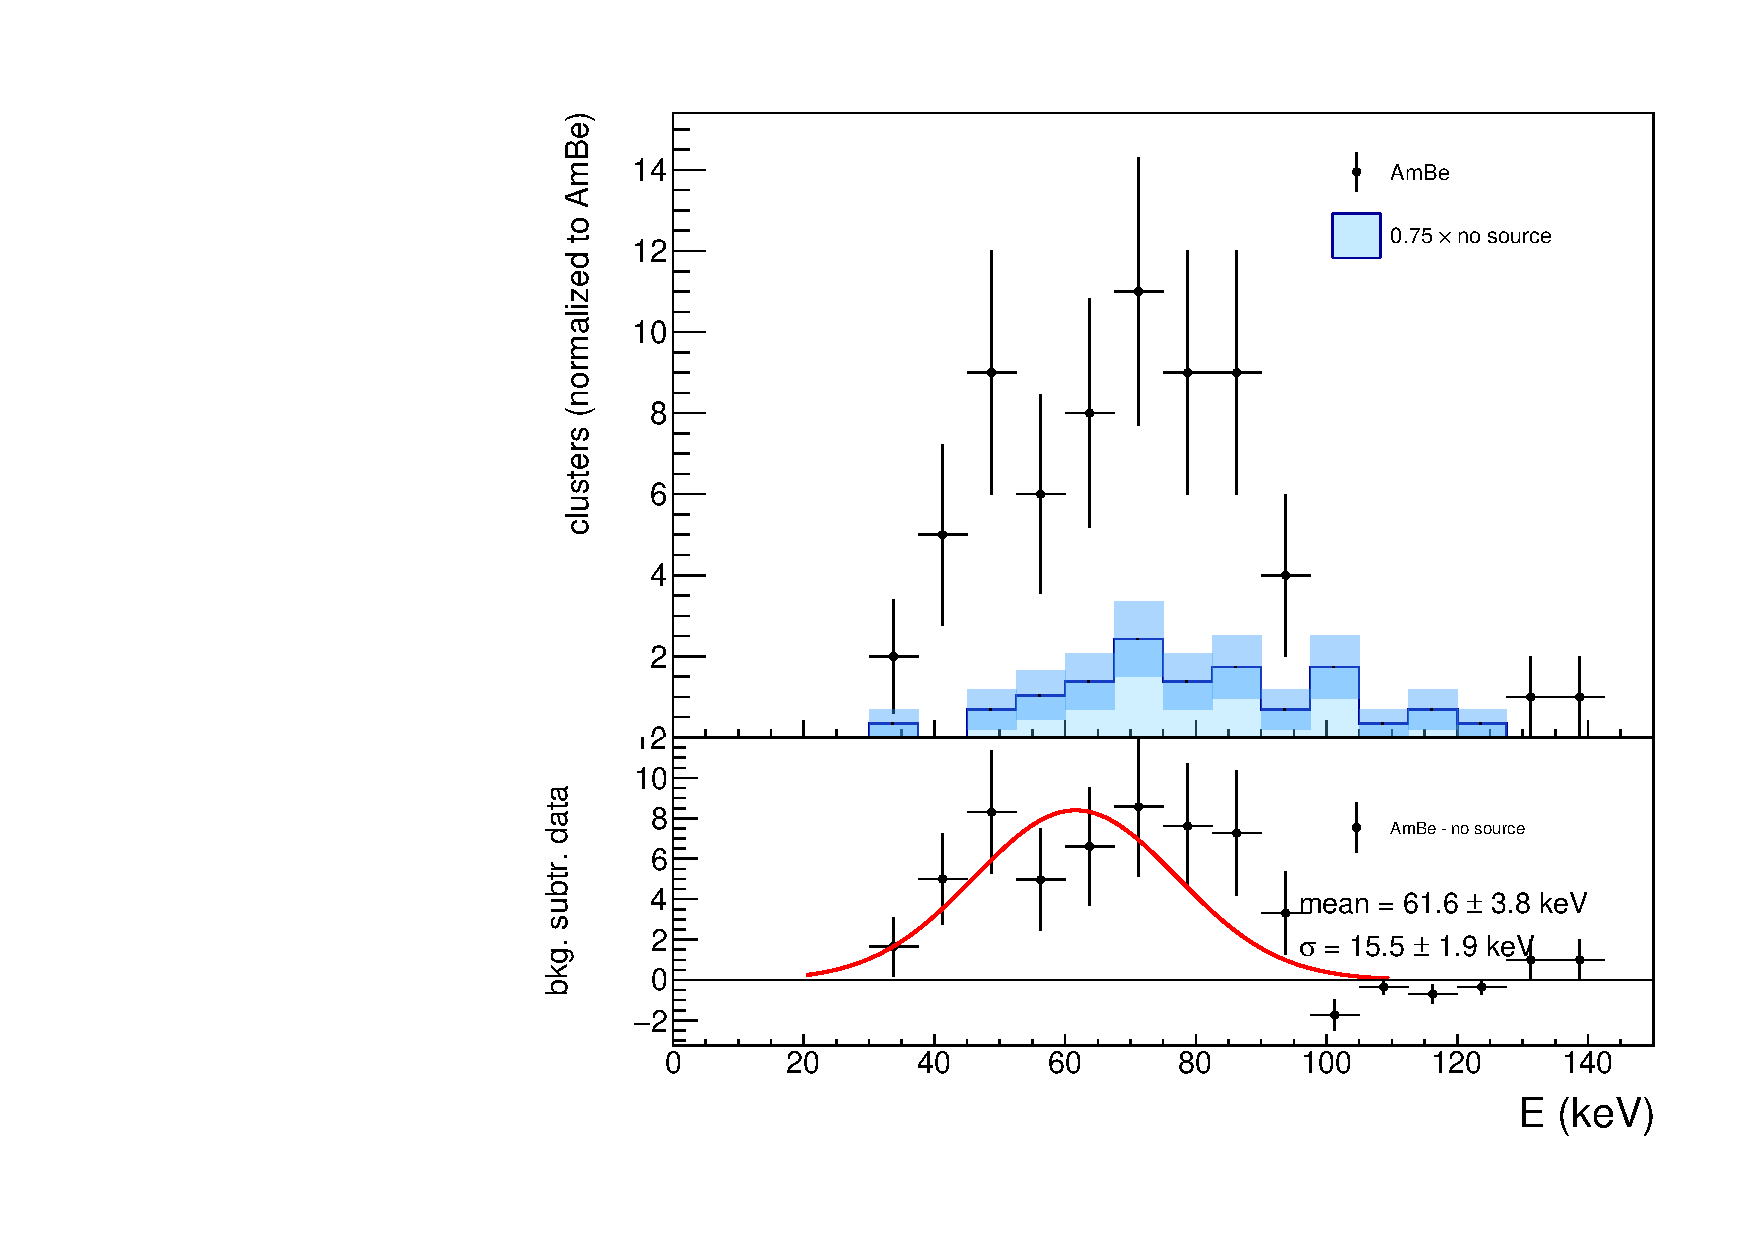
\includegraphics[width=0.60\linewidth]{figures/calintegral_59keV}

  \caption{Calibrated energy spectrum for candidates in the control
    region $PR$, defined in the text. The background-subtracted
    distribution is fitted with a Gaussian PDF, which shows a mean
    value compatible with $E=59\keV$ originated from the $^{241}$Am
    $\gamma$s interaction within the gas. \label{fig:59keV}}

  \end{center}
\end{figure}

\subsection{PMT-based cosmic ray suppression}
An independent information to the light detected by the sCMOS sensor
of the camera is obtained from the PMT pulse, used to trigger the
image shooting. For each image acquired, the corresponding PMT pulse
waveform is recorded.  Tracks from cosmic rays, which typically have a
large angle with respect the cathode plane, as shown in
Fig.~\ref{fig:cosmics} (right), show a broad waveform, characterized
by the different arrival times of the several ionization clusters
produced along the track at different $z$. Conversely, spot-like
signals like \fe deposits or nuclear recoils are characterized by a
short pulse, as shown in Fig.~\ref{fig:waveforms}.
%
\begin{figure}[ht]
  \begin{center}
    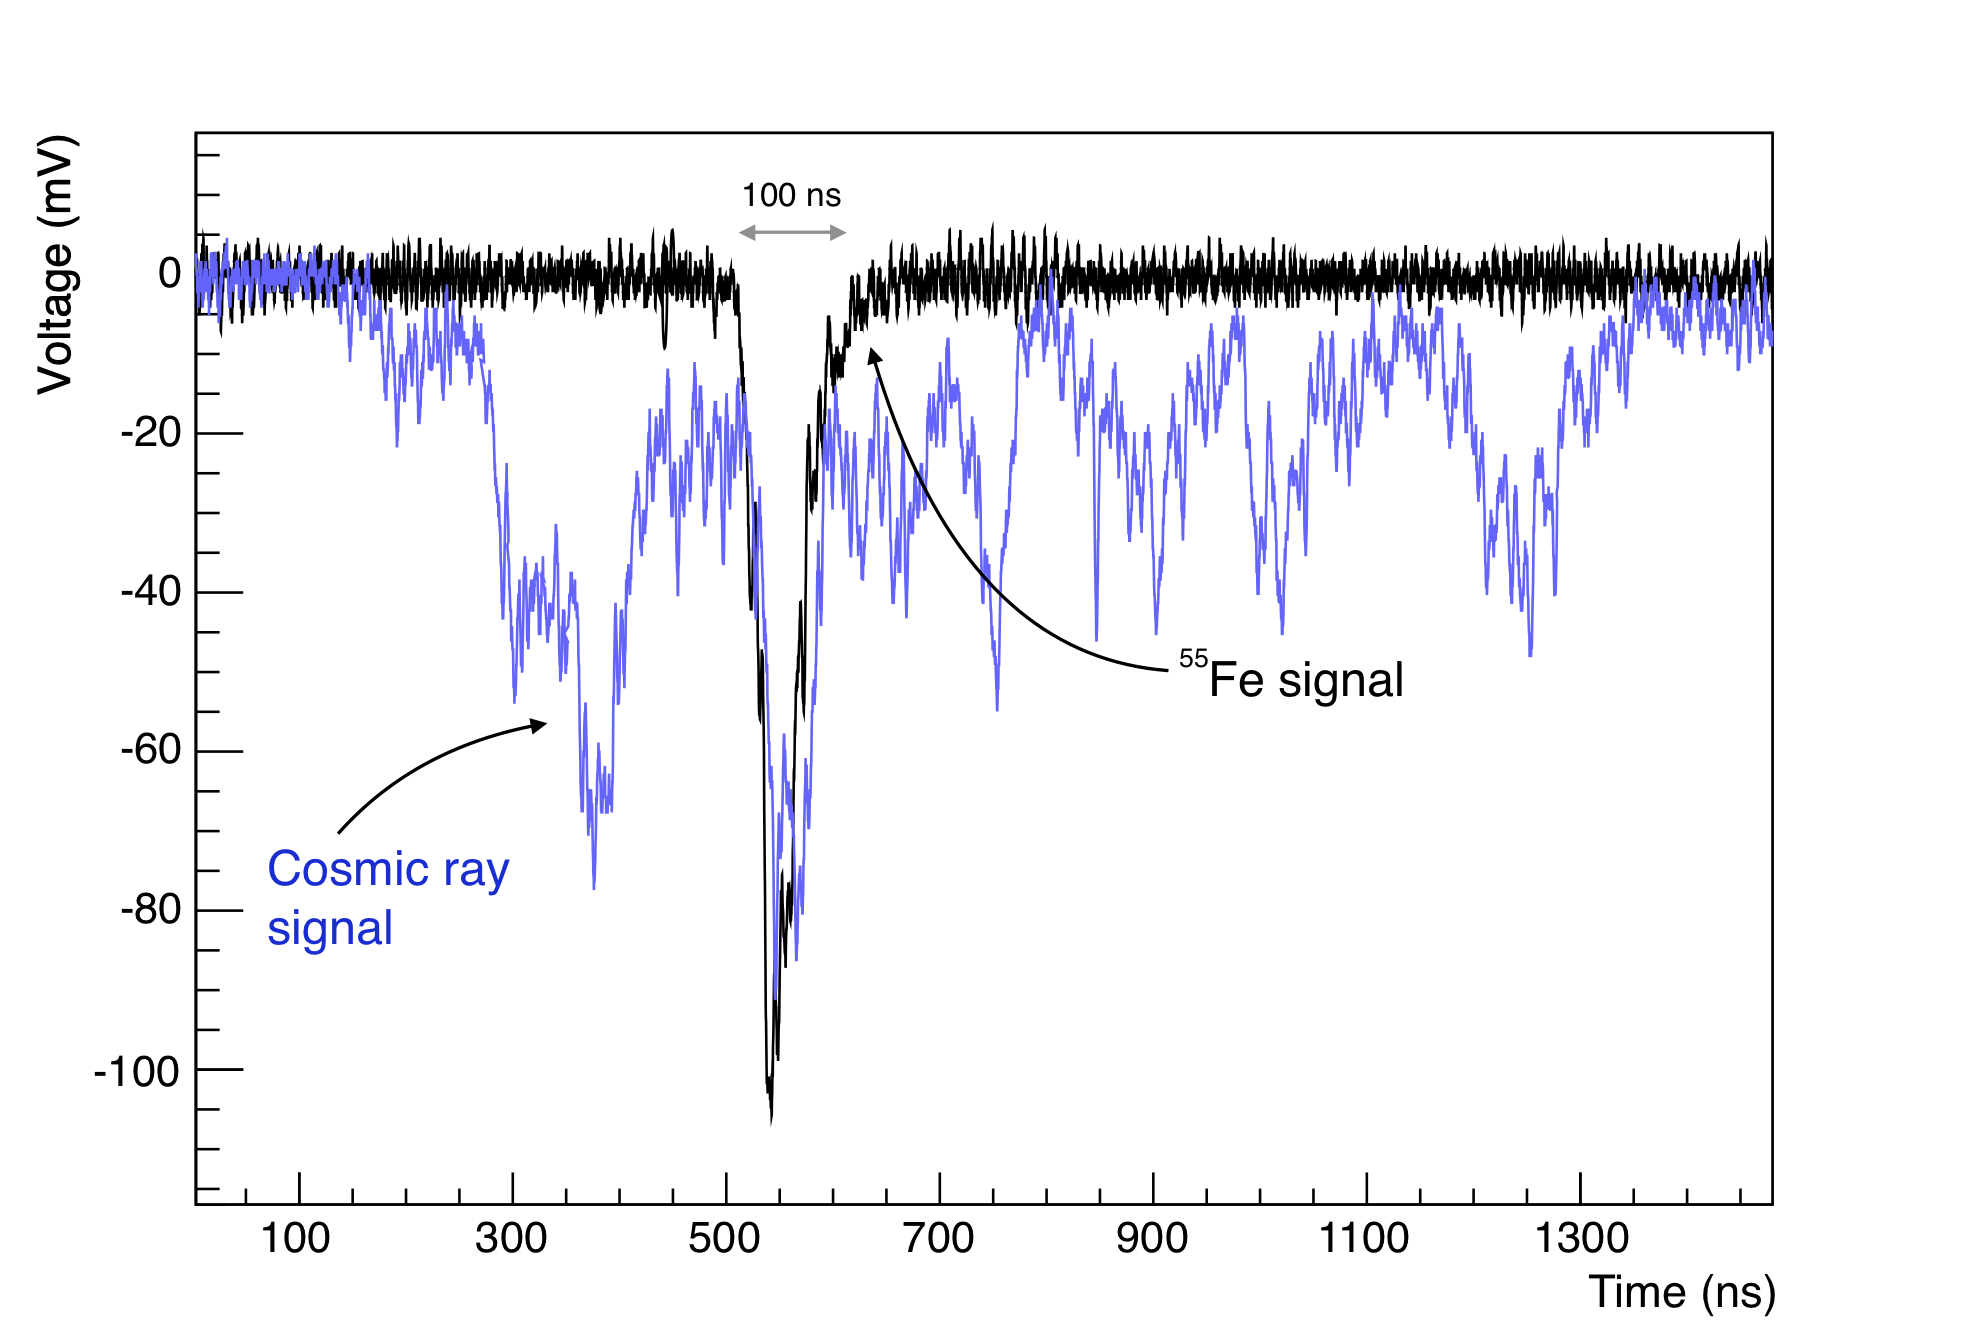
\includegraphics[width=0.69\linewidth]{figures/Waveforms.png}

    \caption{Example of two acquired waveforms: one short pulse
  recorded in presence of \fe radioactive source, together with a long
  signal very likely due to a cosmic ray
  track.  \label{fig:waveforms}}

  \end{center}
\end{figure}

%
The Time Over Threshold (\textit{TOT}) of the PMT pulse was measured,
and is shown in Fig.~\ref{fig:pmttot}. It can be seen from the region
around 270\unit{ns}, dominated by the cosmic rays also in the data
with the \ambe source, that the trigger scale factor
$\varepsilon_{SF}$ also holds for the PMT event rate.
%
\begin{figure}[ht]
  \begin{center}
  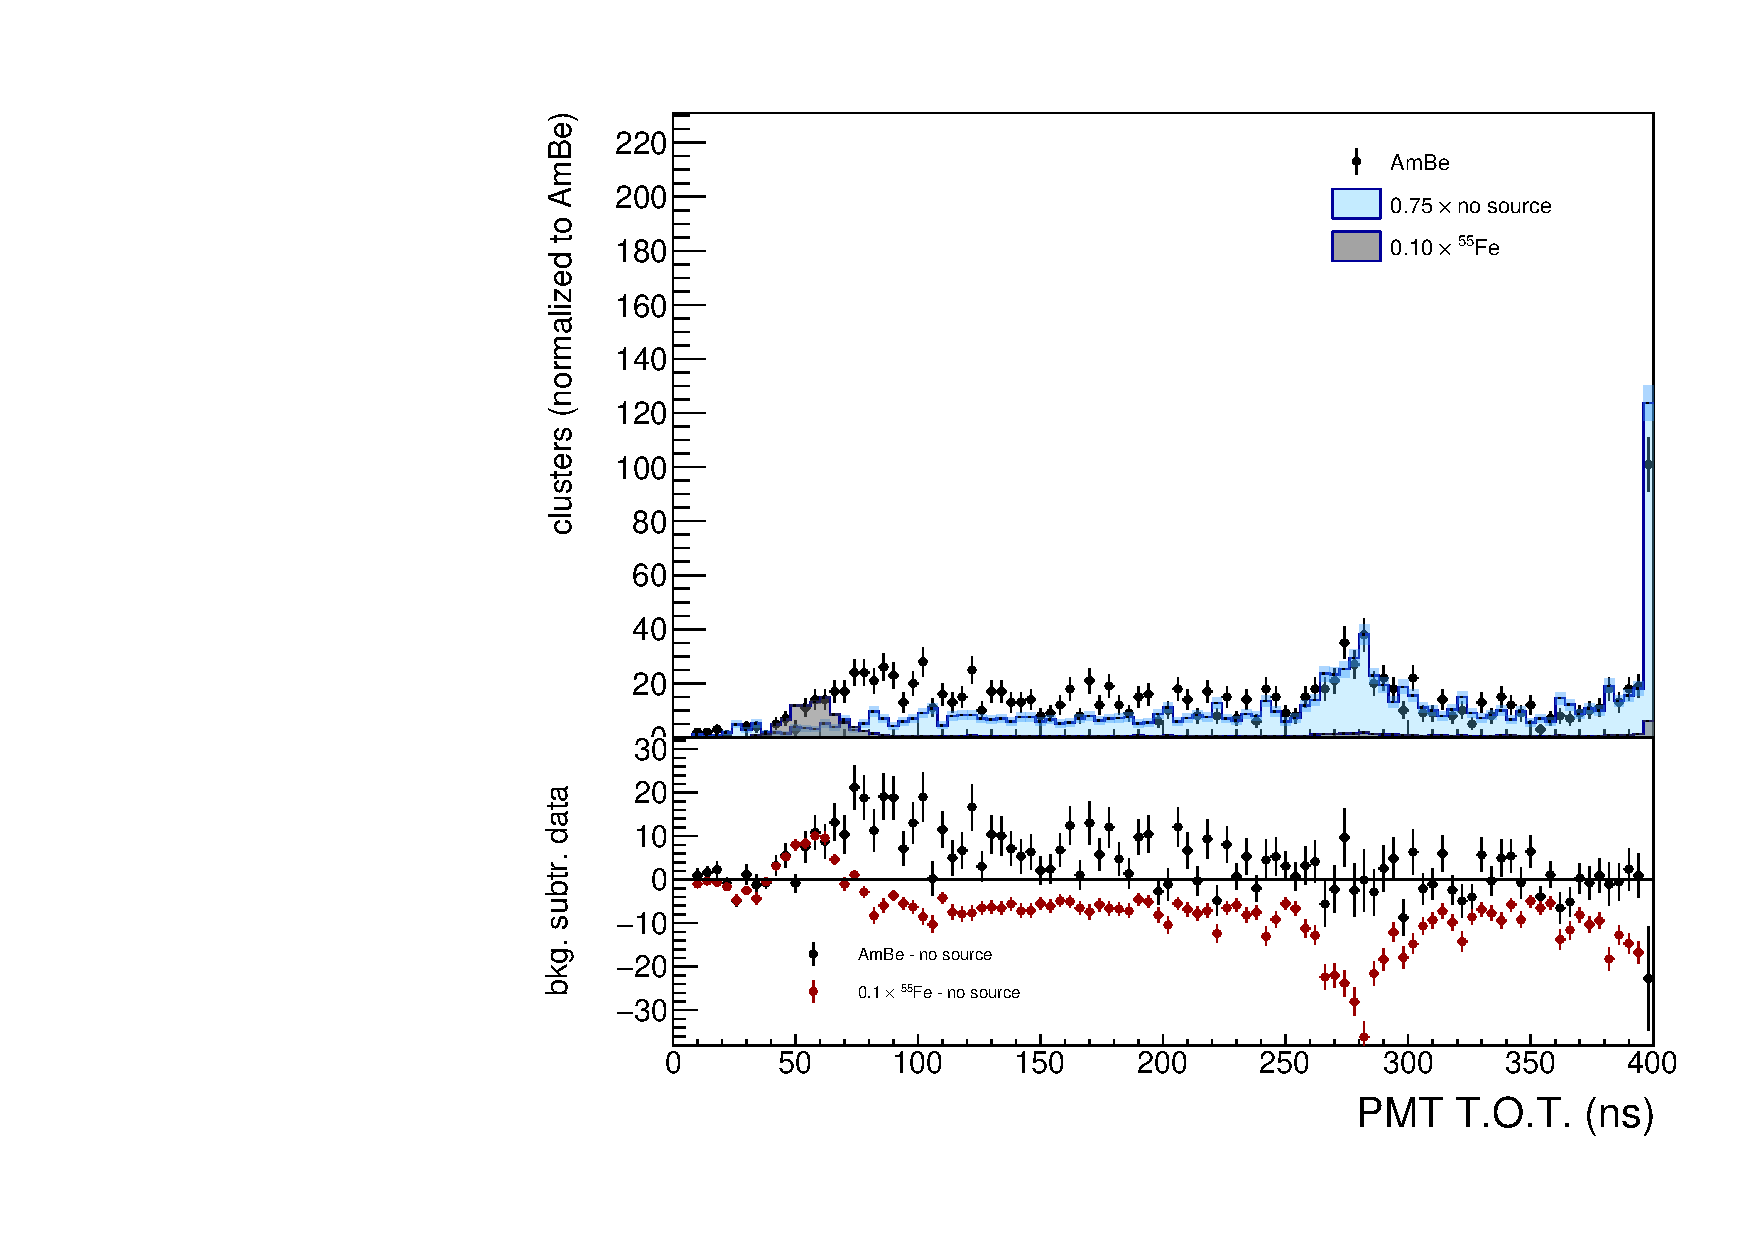
\includegraphics[width=0.45\linewidth]{figures/pmt_tot}

   \caption{PMT waveform time over threshold ($TOT$).  The last bin
    integrates all the events with $TOT>400$\unit{ns}. Filled points
    represent data with \ambe source, dark gray (light blue)
    distribution represents data with \fe source (no source).  The
    normalization of data without source is to the same exposure time
    of the \ambe one, with trigger scale factor $\varepsilon_{SF}$
    applied. For the data with \fe, a scaling factor of one tenth is
    applied for clearness, given the larger activity of this
    source. \label{fig:pmttot}}

  \end{center}
\end{figure}
%
As expected, spot-like clusters (in 3D) correspond to a short pulse in
the PMT, while cosmic ray tracks have a much larger pulse. The
contribution of cosmic ray tracks is clearly visible in the data with
radioactive sources. A selection on this variable is helpful to
further reject residual cosmic rays background present in the \ambe or
\fe data, in particular tracks which may have been split in multiple
superclusters, like the case shown in Fig.~\ref{fig:super_clusters2}
(bottom), and thus passing the above preselection on the cluster
shapes. A selection $TOT<250$\unit{ns} is then imposed.  It has an efficiency of 98\% on cluster candidates in
\ambe data (after background subtraction), while it is only 80\%
efficient on data with \fe source.  The light density, and the energy
spectrum, after the full preselection, is shown in
Fig.~\ref{fig:presel}.
%
\begin{figure}[ht]
  \begin{center}
  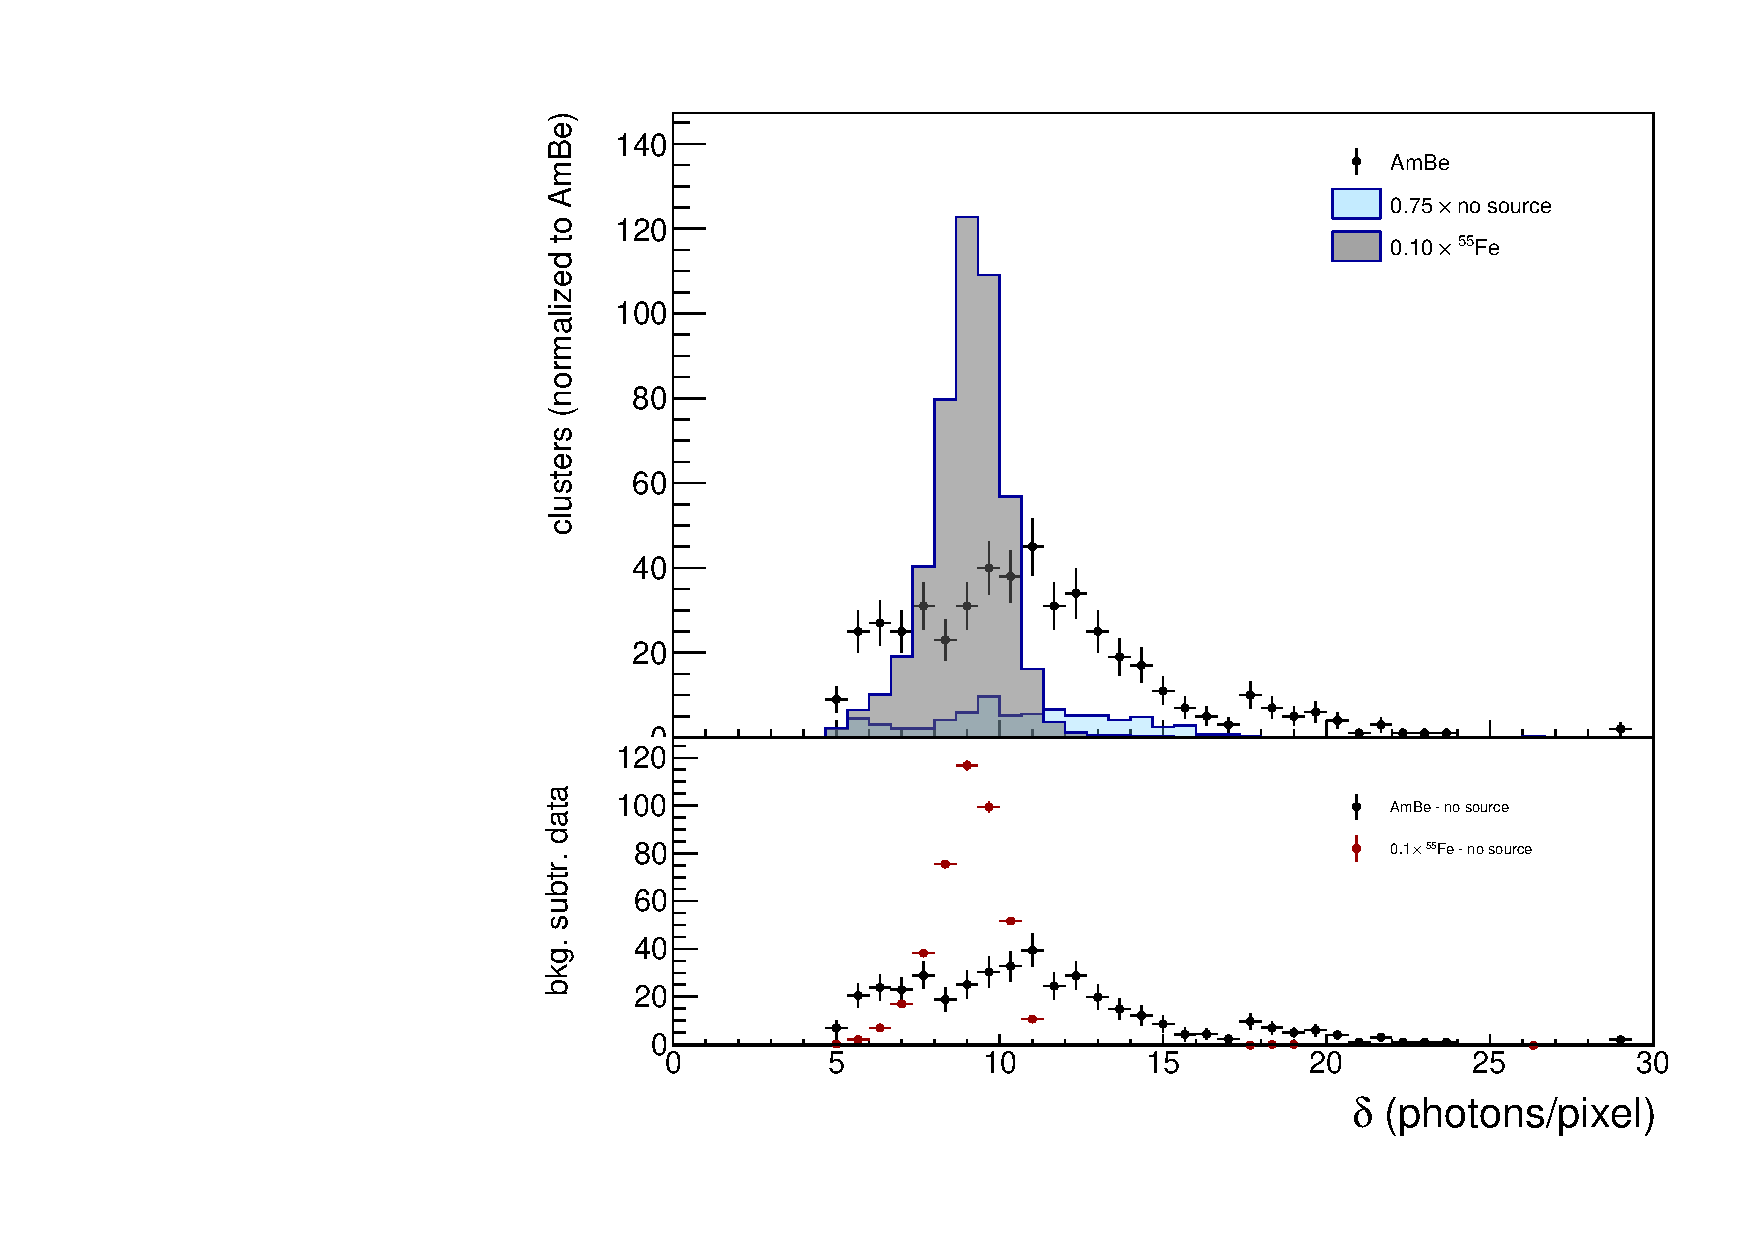
\includegraphics[width=0.45\linewidth]{figures/density_fullSel}
  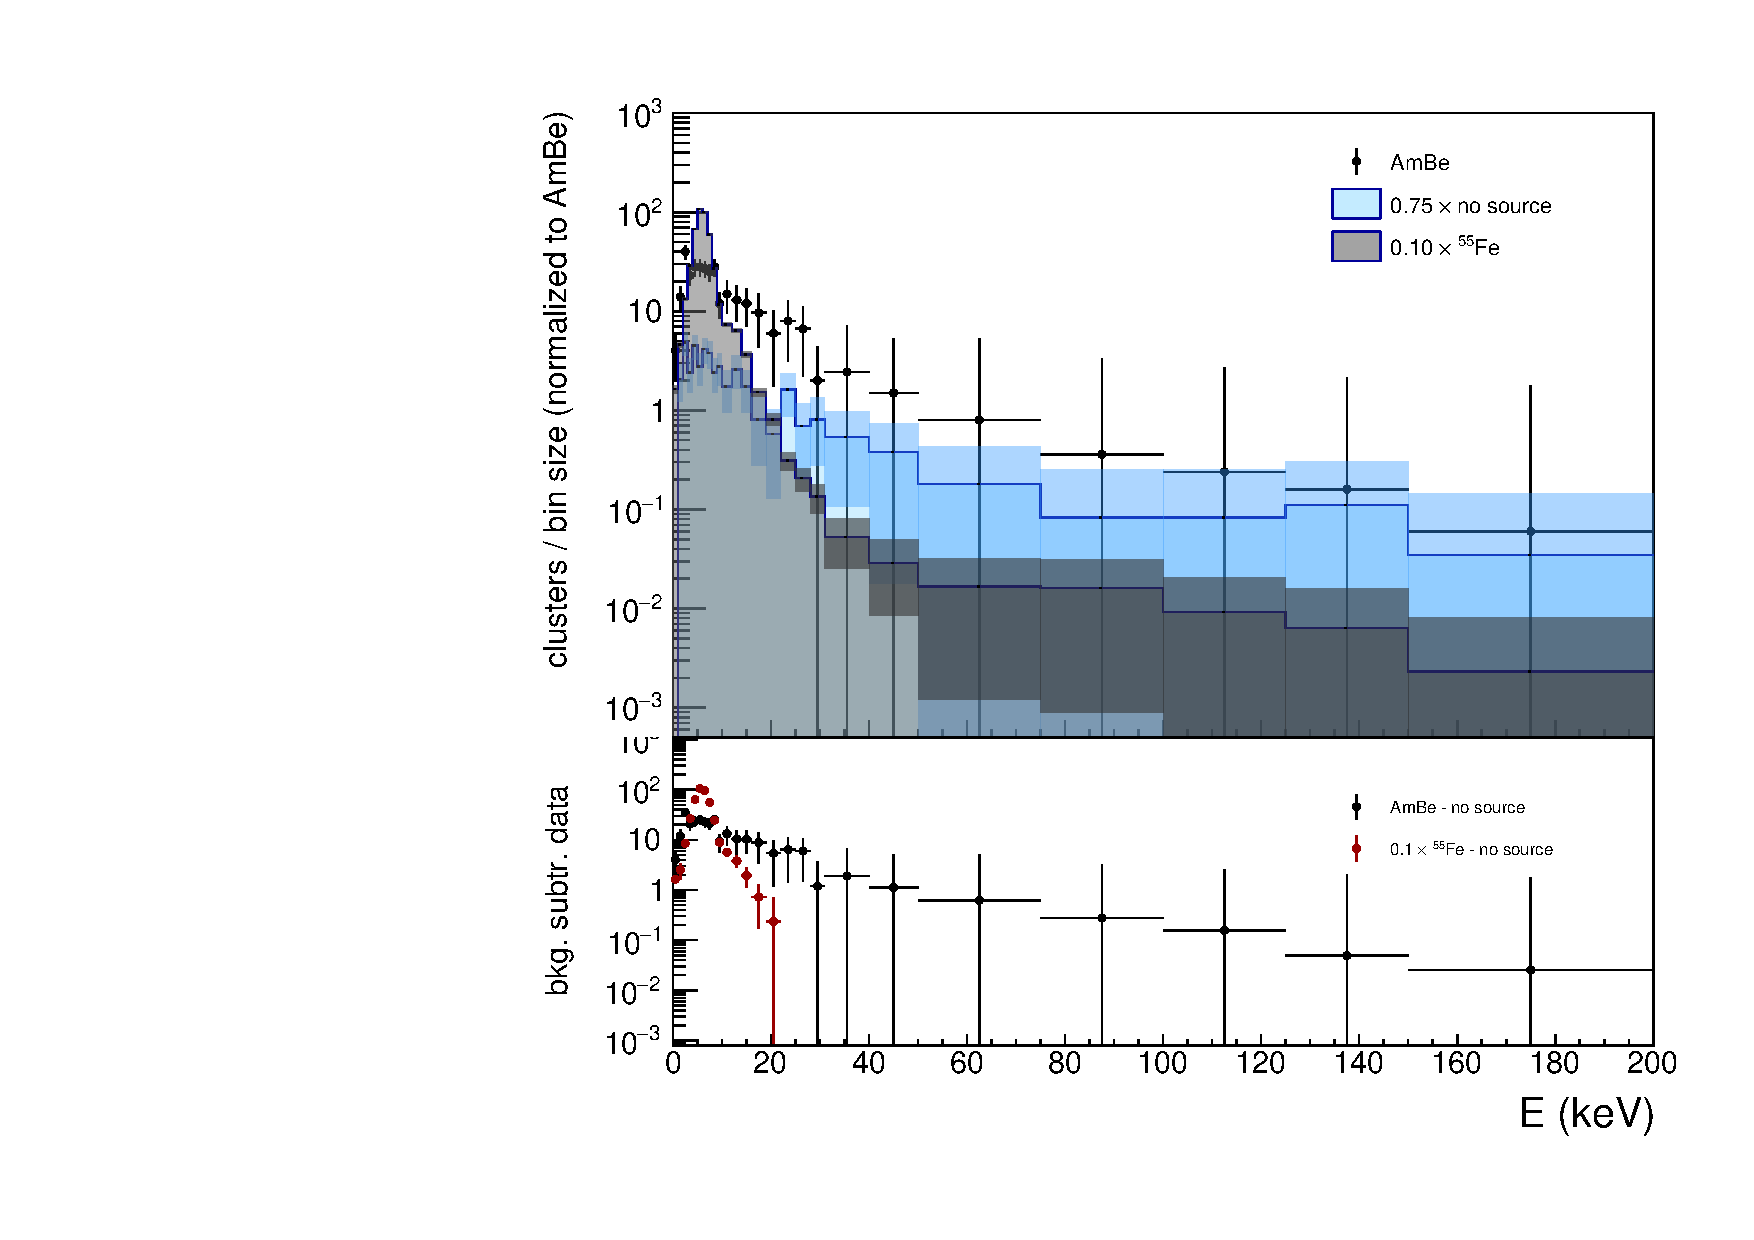
\includegraphics[width=0.45\linewidth]{figures/energy_fullSel}

  \caption{Supercluster light density $\delta$ (left) and calibrated
    energy $E$ (right), after the preselection and cosmic ray
    suppression described in the text to select nuclear recoil
    candidates. Filled points represent data with \ambe source, dark
    gray (light blue) distribution represents data with \fe source
    (no-source).  The normalization of no-source data is to the same
    exposure time of the \ambe data, with the trigger scale factor
    $\varepsilon_{SF}$ applied. For the data with \fe, a scaling
    factor of one tenth is applied for clearness, given the larger
    activity of this source.  \label{fig:presel}}

  \end{center}
\end{figure}

\subsection{Light density and  \fe events rejection}
The light density distribution, after the above preselection and
cosmic ray suppression, appear to be different among the data
with \ambe source, data with \fe source, and data without any
artificial source.  The cosmic-background-subtracted distributions of
$\delta$ in \ambe data and \fe data, shown in the bottom panel of
Fig.~\ref{fig:presel} (left), are used to evaluate a curve of electron
recoils rejection ($1-\varepsilon^\delta_{B}$) as a function of signal
efficiency ($\varepsilon^\delta_{S}$), obtained varying the selection
on $\delta$. This is shown in Fig.~\ref{fig:roc}.  The same procedure
could be applied to estimate the rejection factor against the cosmic
ray induced background, but this is not shown because of the limited
size of the no-source data. This kind of background will however be
negligible when operating the detector underground. This is shown in
Fig.~\ref{fig:roc}. While this cut-based approach is minimalist, and
could be improved by profiting of the correlations among $\delta$ and
the observables used in the preselection in a more sophisticated
multivariate analysis, it shows that a good rejection factor of
electron recoils at $E=5.9\keV$ can be obtained.
%
\begin{figure}[ht]
  \begin{center}
  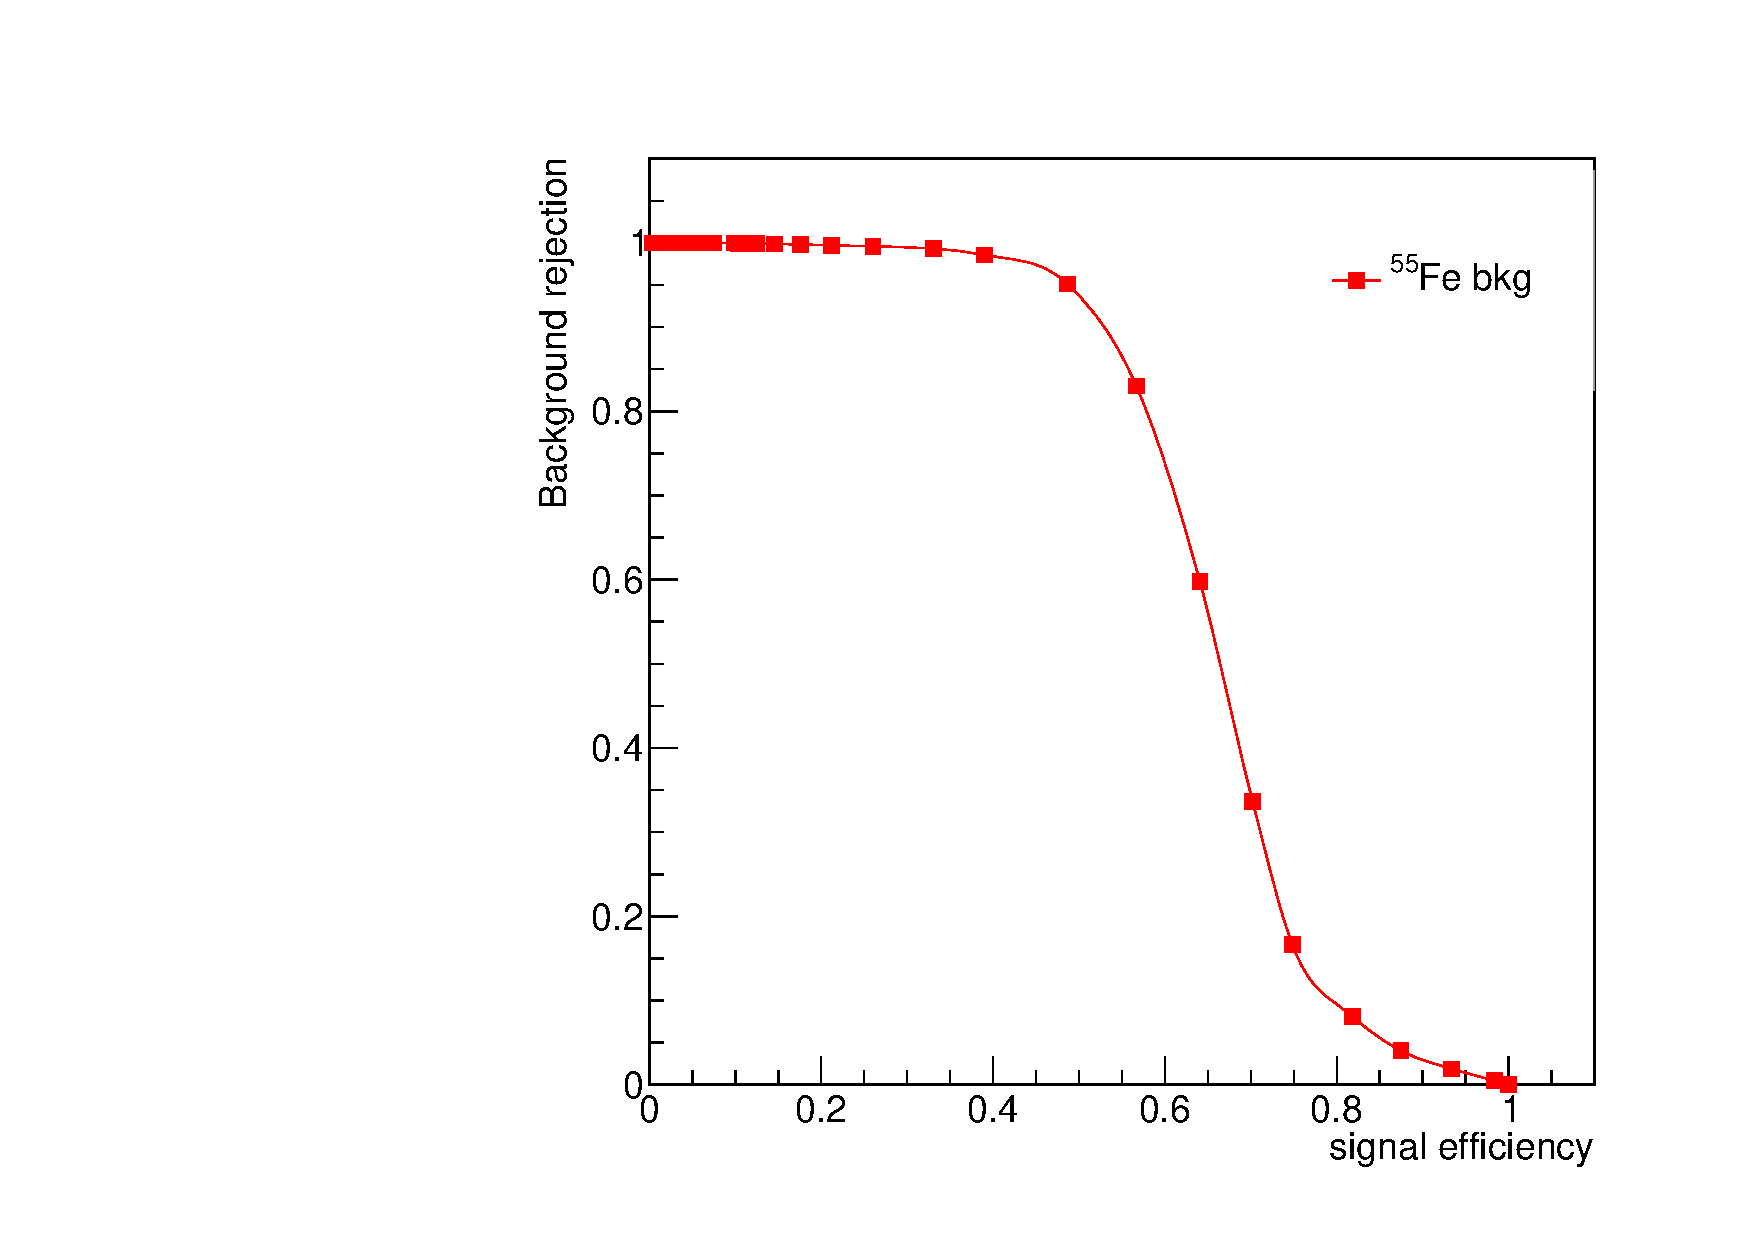
\includegraphics[width=0.45\linewidth]{figures/density_roc}

  \caption{Background rejection as a function of the signal
    efficiency, varying the selection on the $\delta$ variable in data
    with either \fe (background sample) or \ambe (signal sample)
    sources.  \label{fig:roc}}

  \end{center}
\end{figure}
%

 Table~\ref{tab:roc} shows then the
full signal efficiency and electrons rejection factor for two example
working points, $\mathrm{WP}_{40}$ and $\mathrm{WP}_{50}$, having 40\%
and 50\% signal efficiency for the selection on $\delta$. They
correspond to a selection $\delta>11$ and $\delta>10$, respectively.


\begin{table*}[t]
\caption{Signal (nuclear recoils) and background (electron recoils) efficiency for
  two different selections on $\delta$.\label{tab:roc}}
\vspace{10pt}
\normalsize
\centering
\begin{tabular}{l c c c | c c c }
  \hline\hline
  working point & \multicolumn{3}{c}{Signal efficiency} & \multicolumn{3}{c}{Background efficiency} \\
  \hline
  & $\varepsilon_{S}^{presel}$ & $\varepsilon_{S}^{\delta}$ & $\varepsilon_{S}^{total}$ & $\varepsilon_{B}^{presel}$ & $\varepsilon_{B}^{\delta}$ & $\varepsilon_{B}^{total}$ \\
  \hline
  $\mathrm{WP}_{50}$  & 0.98                        & 0.51                      & 0.50                     & 0.70                     & 0.050                     & 0.035 \\
  $\mathrm{WP}_{40}$  & 0.98                        & 0.41                      & 0.40                     & 0.70                     & 0.012                     & 0.008 \\
  \hline\hline
\end{tabular}
\end{table*}

\subsection{Signal Energy Spectrum and efficiency}
The energy spectrum for the candidates with $\varepsilon_{S}^{total}$
= 50\% in the \ambe sample is shown in Fig.~\ref{fig:fullsel_effi}
(left). With the full $\mathrm{WP}_{50}$ selection, the signal
efficiency is computed for both the example working points in bins of
energy. The electron recoil efficiency, $\varepsilon_{B}^{total}$,
represents a $\gamma$ background efficiency at a fixed energy
$E=6\keV$, that is close to the \fe emitted photon energy. For the
$\mathrm{WP}_{50}$, the efficiency for very low-energy recoils,
$E=6\keV$, is still 18\%, dropping to almost zero at $E\lesssim4\keV$.

\begin{figure}[ht]
  \begin{center}
    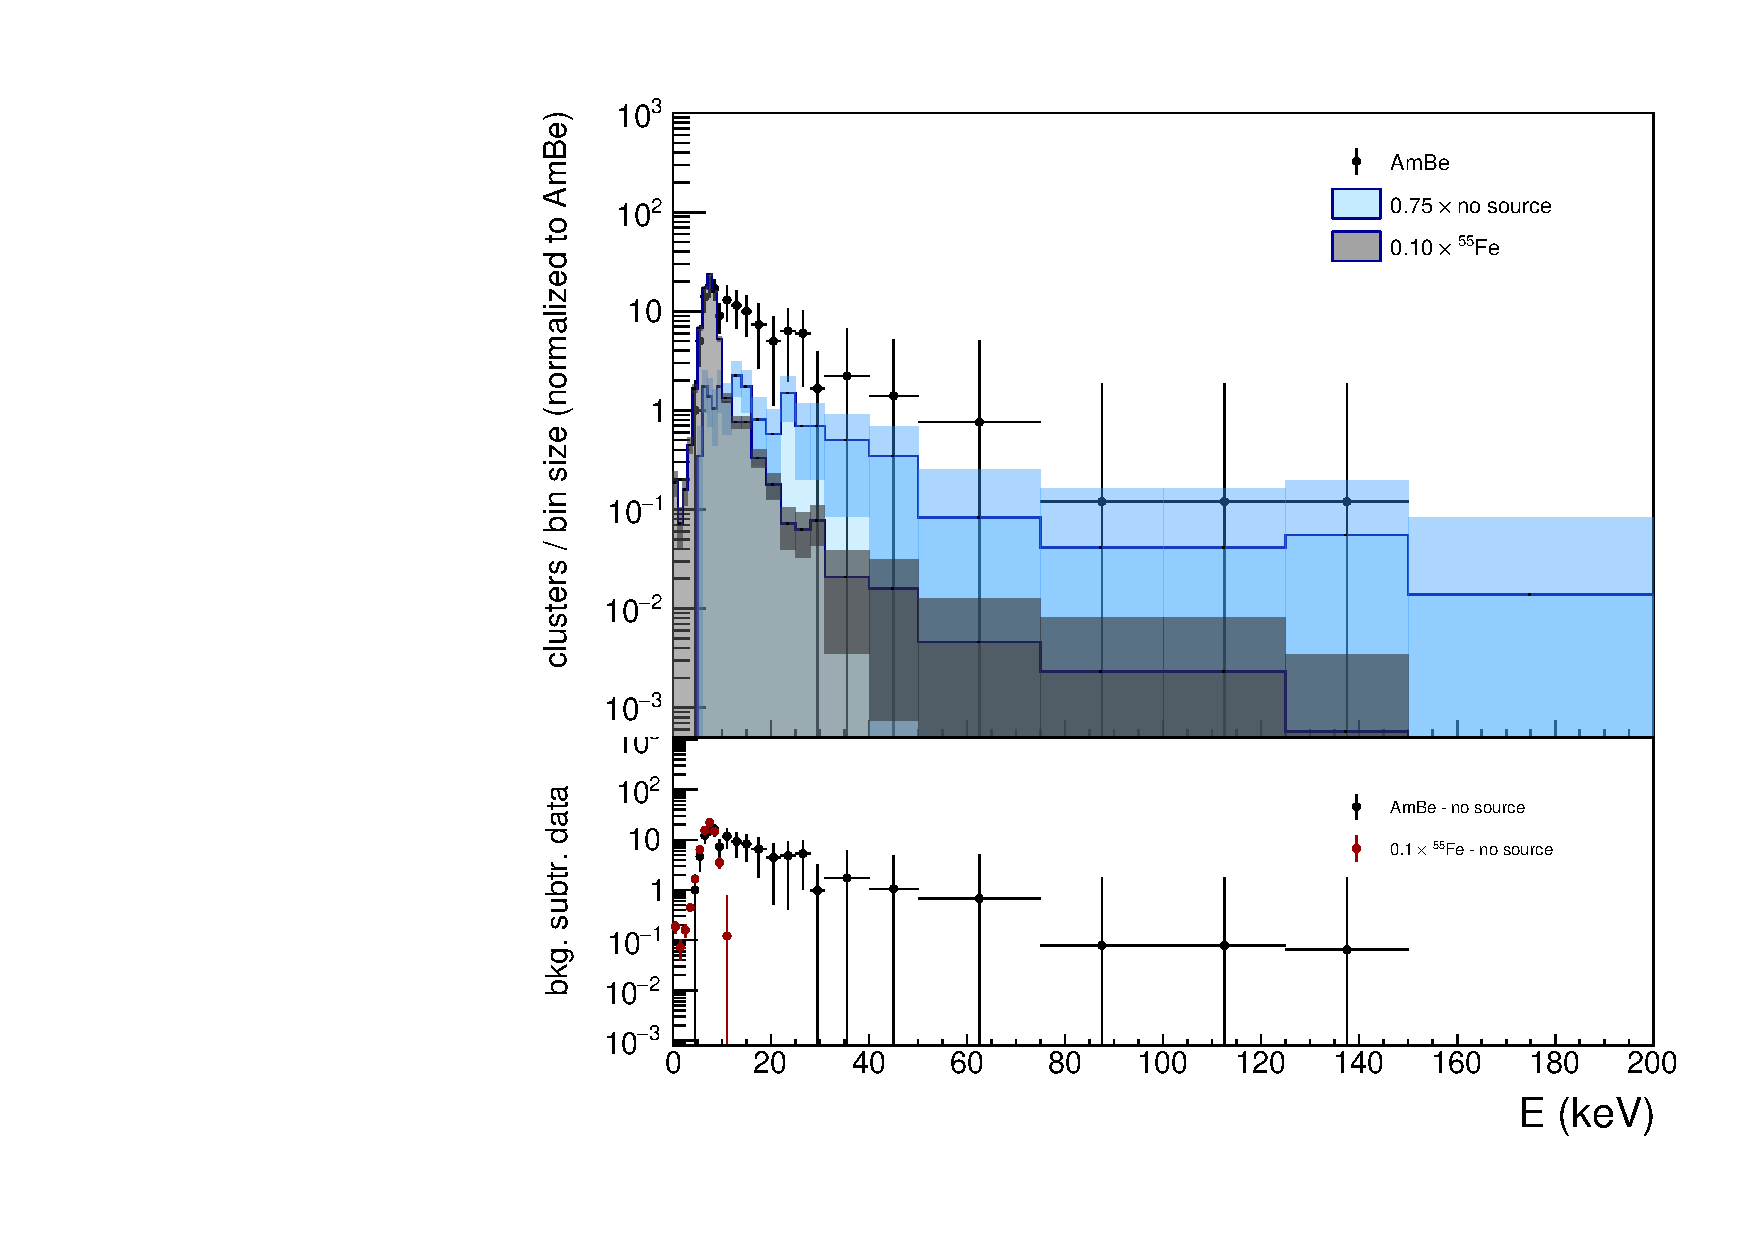
\includegraphics[width=0.45\linewidth]{figures/energyFull_WP50}
    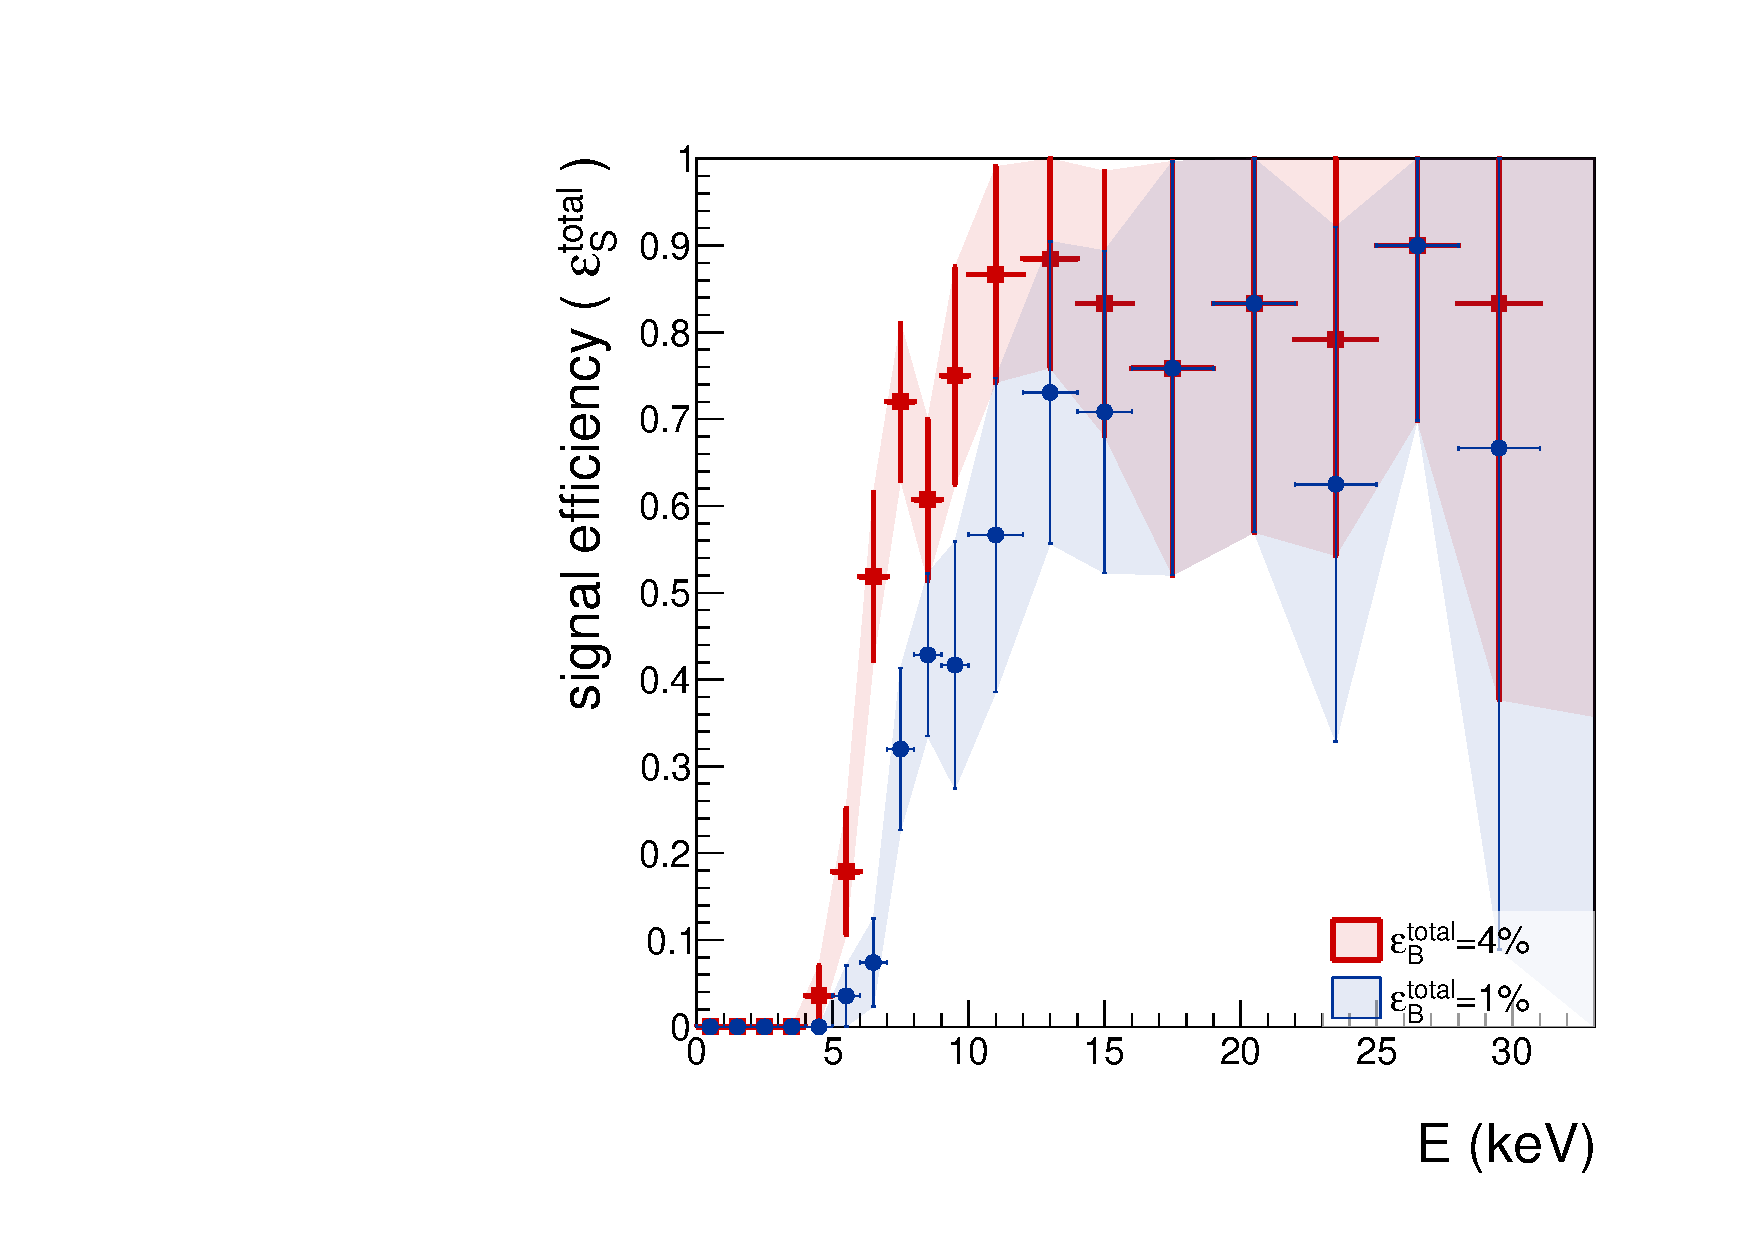
\includegraphics[width=0.45\linewidth]{figures/energyFull_effi}

    \caption{Left: supercluster calibrated energy $E$ (left), after the
      full selection, which includes $\delta>10$, 50\% efficient on
      signal, to select nuclear recoil candidates. Filled points
      represent data with \ambe source, dark gray (light blue)
      distribution represents   \fe source (no-source) data.  The
      normalization of no-source  data  is to the same exposure
      time of the \ambe data, with the trigger scale factor
      $\varepsilon_{SF}$ applied. For the  \fe data, a scaling
      factor of one tenth is applied for clearness, given the larger
      activity of this source. Right: efficiency for nuclear recoil
      candidates as a function of energy, estimated on \ambe data, for
      two example selections, described in the text, having either 4\%
      or 1\% efficiency on electron recoils at
      $E=6\keV$. \label{fig:fullsel_effi}}

  \end{center}
\end{figure}

Two candidate  nuclear recoils images, fulfilling the 
$\mathrm{WP}_{50}$ selection  (with a light density $\delta\gtrsim10$
photons/pixels and with energies of 5.2 and 6.0\keV)  are shown in
Fig.~\ref{fig:lowEnergyNR}. The displayed images are a portion of the full-resolution frame, after the pedestal subtraction.

\begin{figure}[ht]
  \begin{center}
  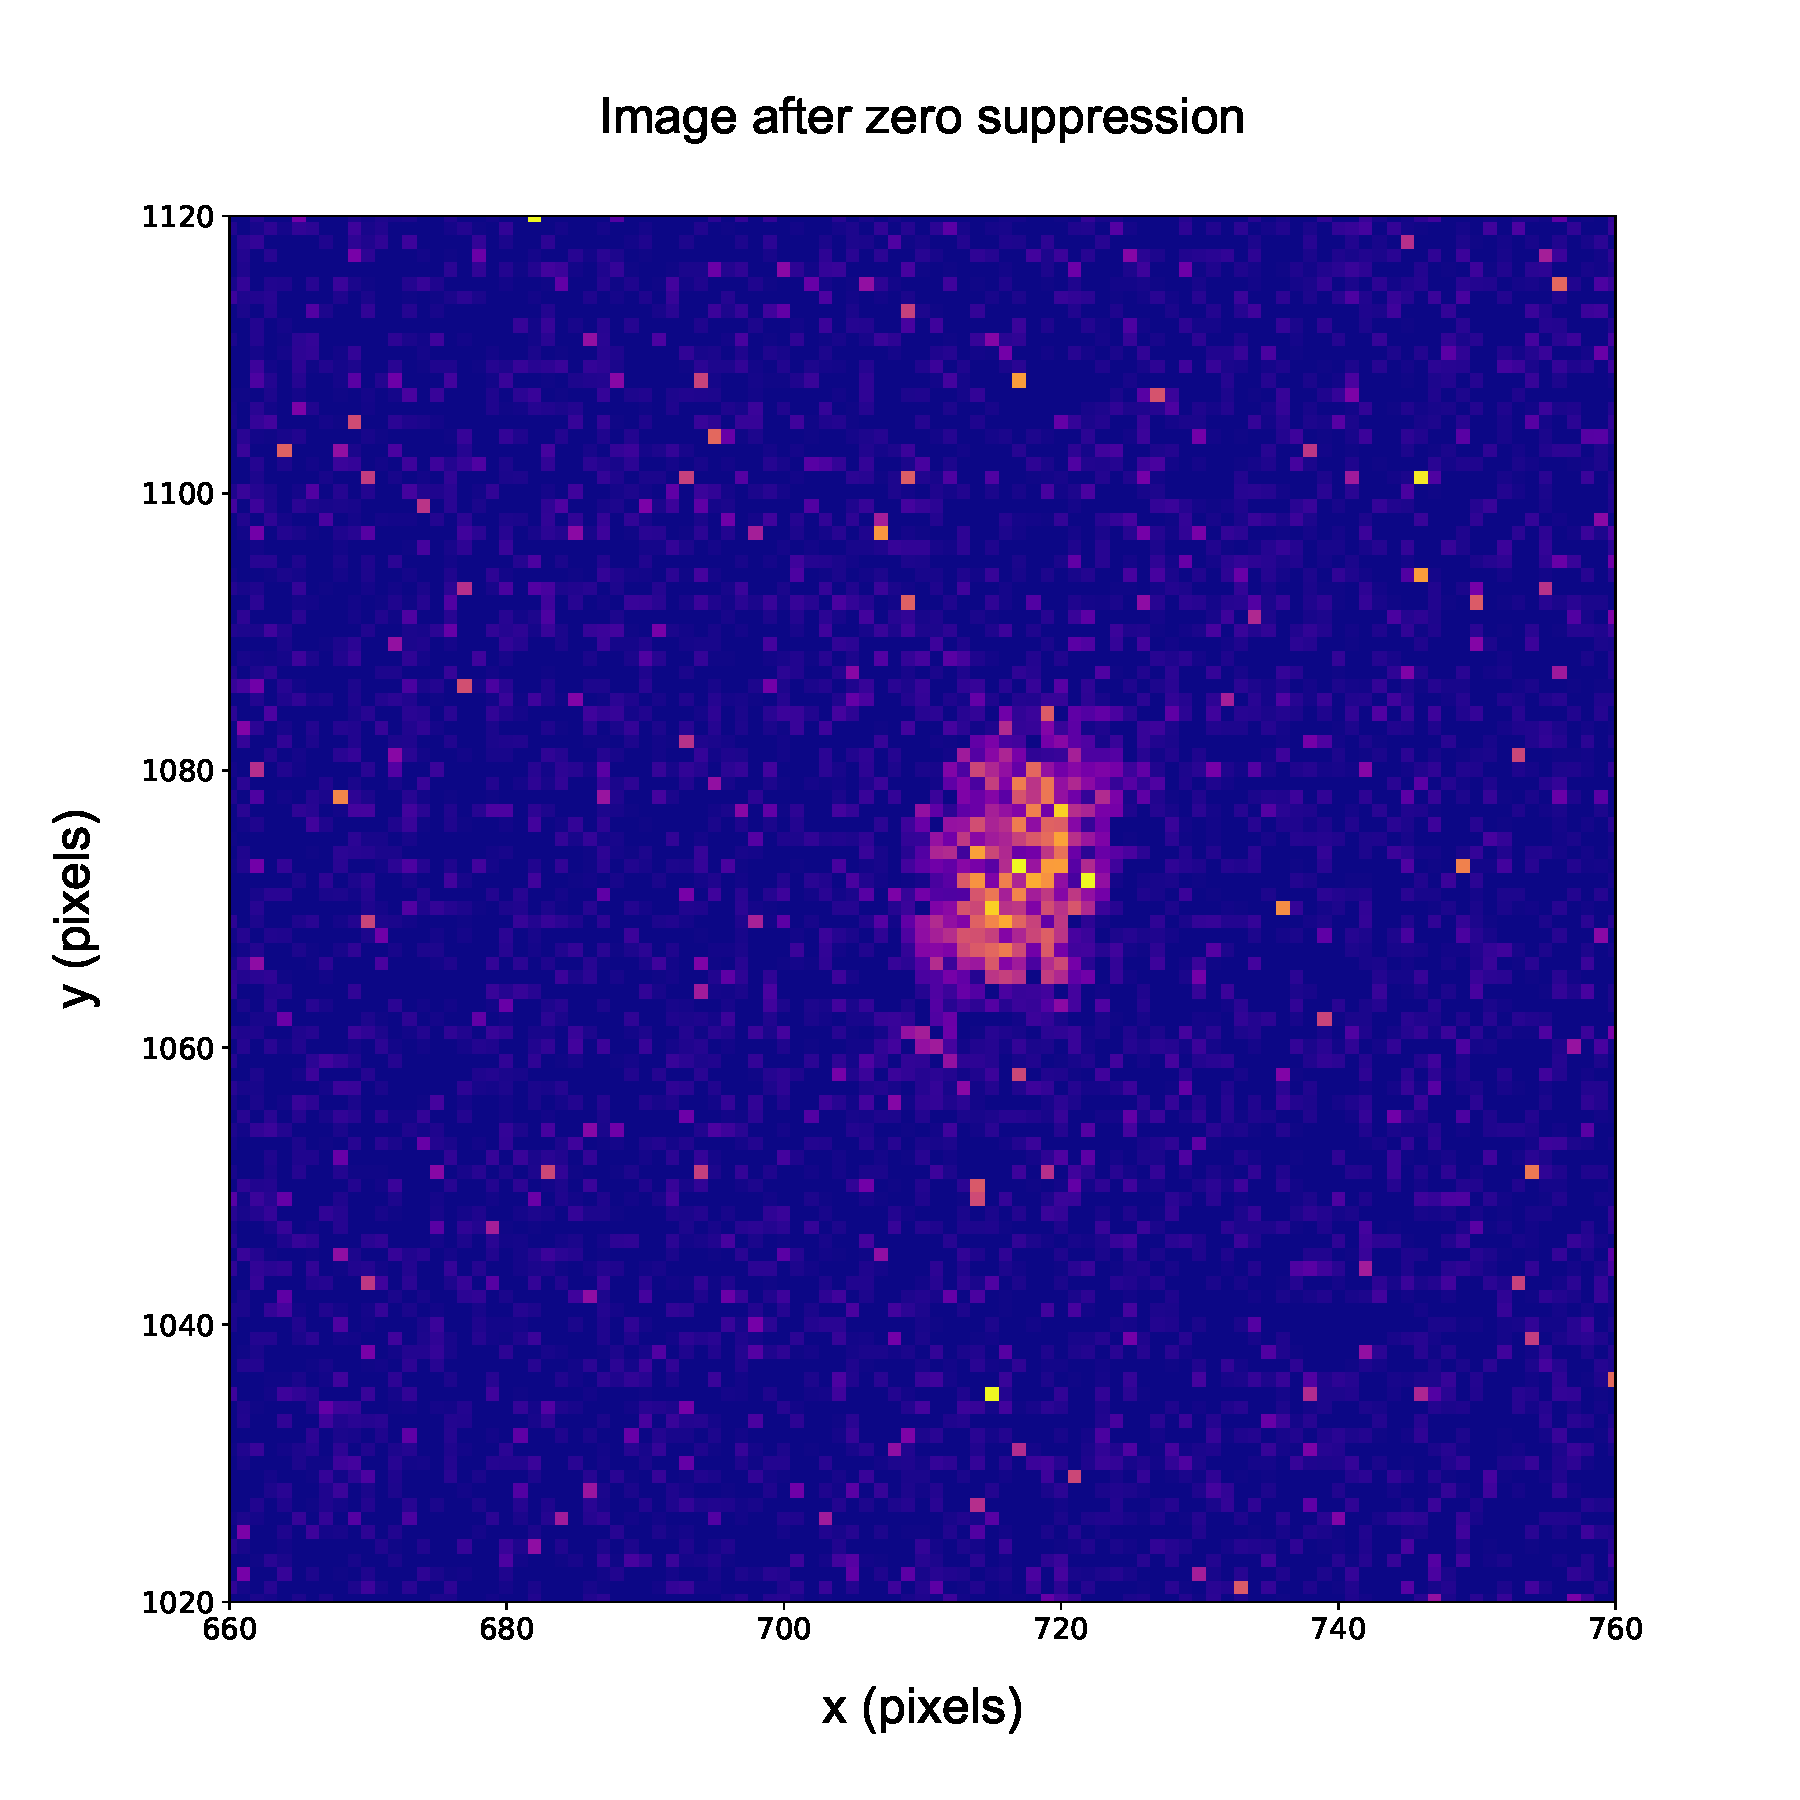
\includegraphics[width=0.49\linewidth]{figures/pic_run02097_ev59_oriIma_paper}
  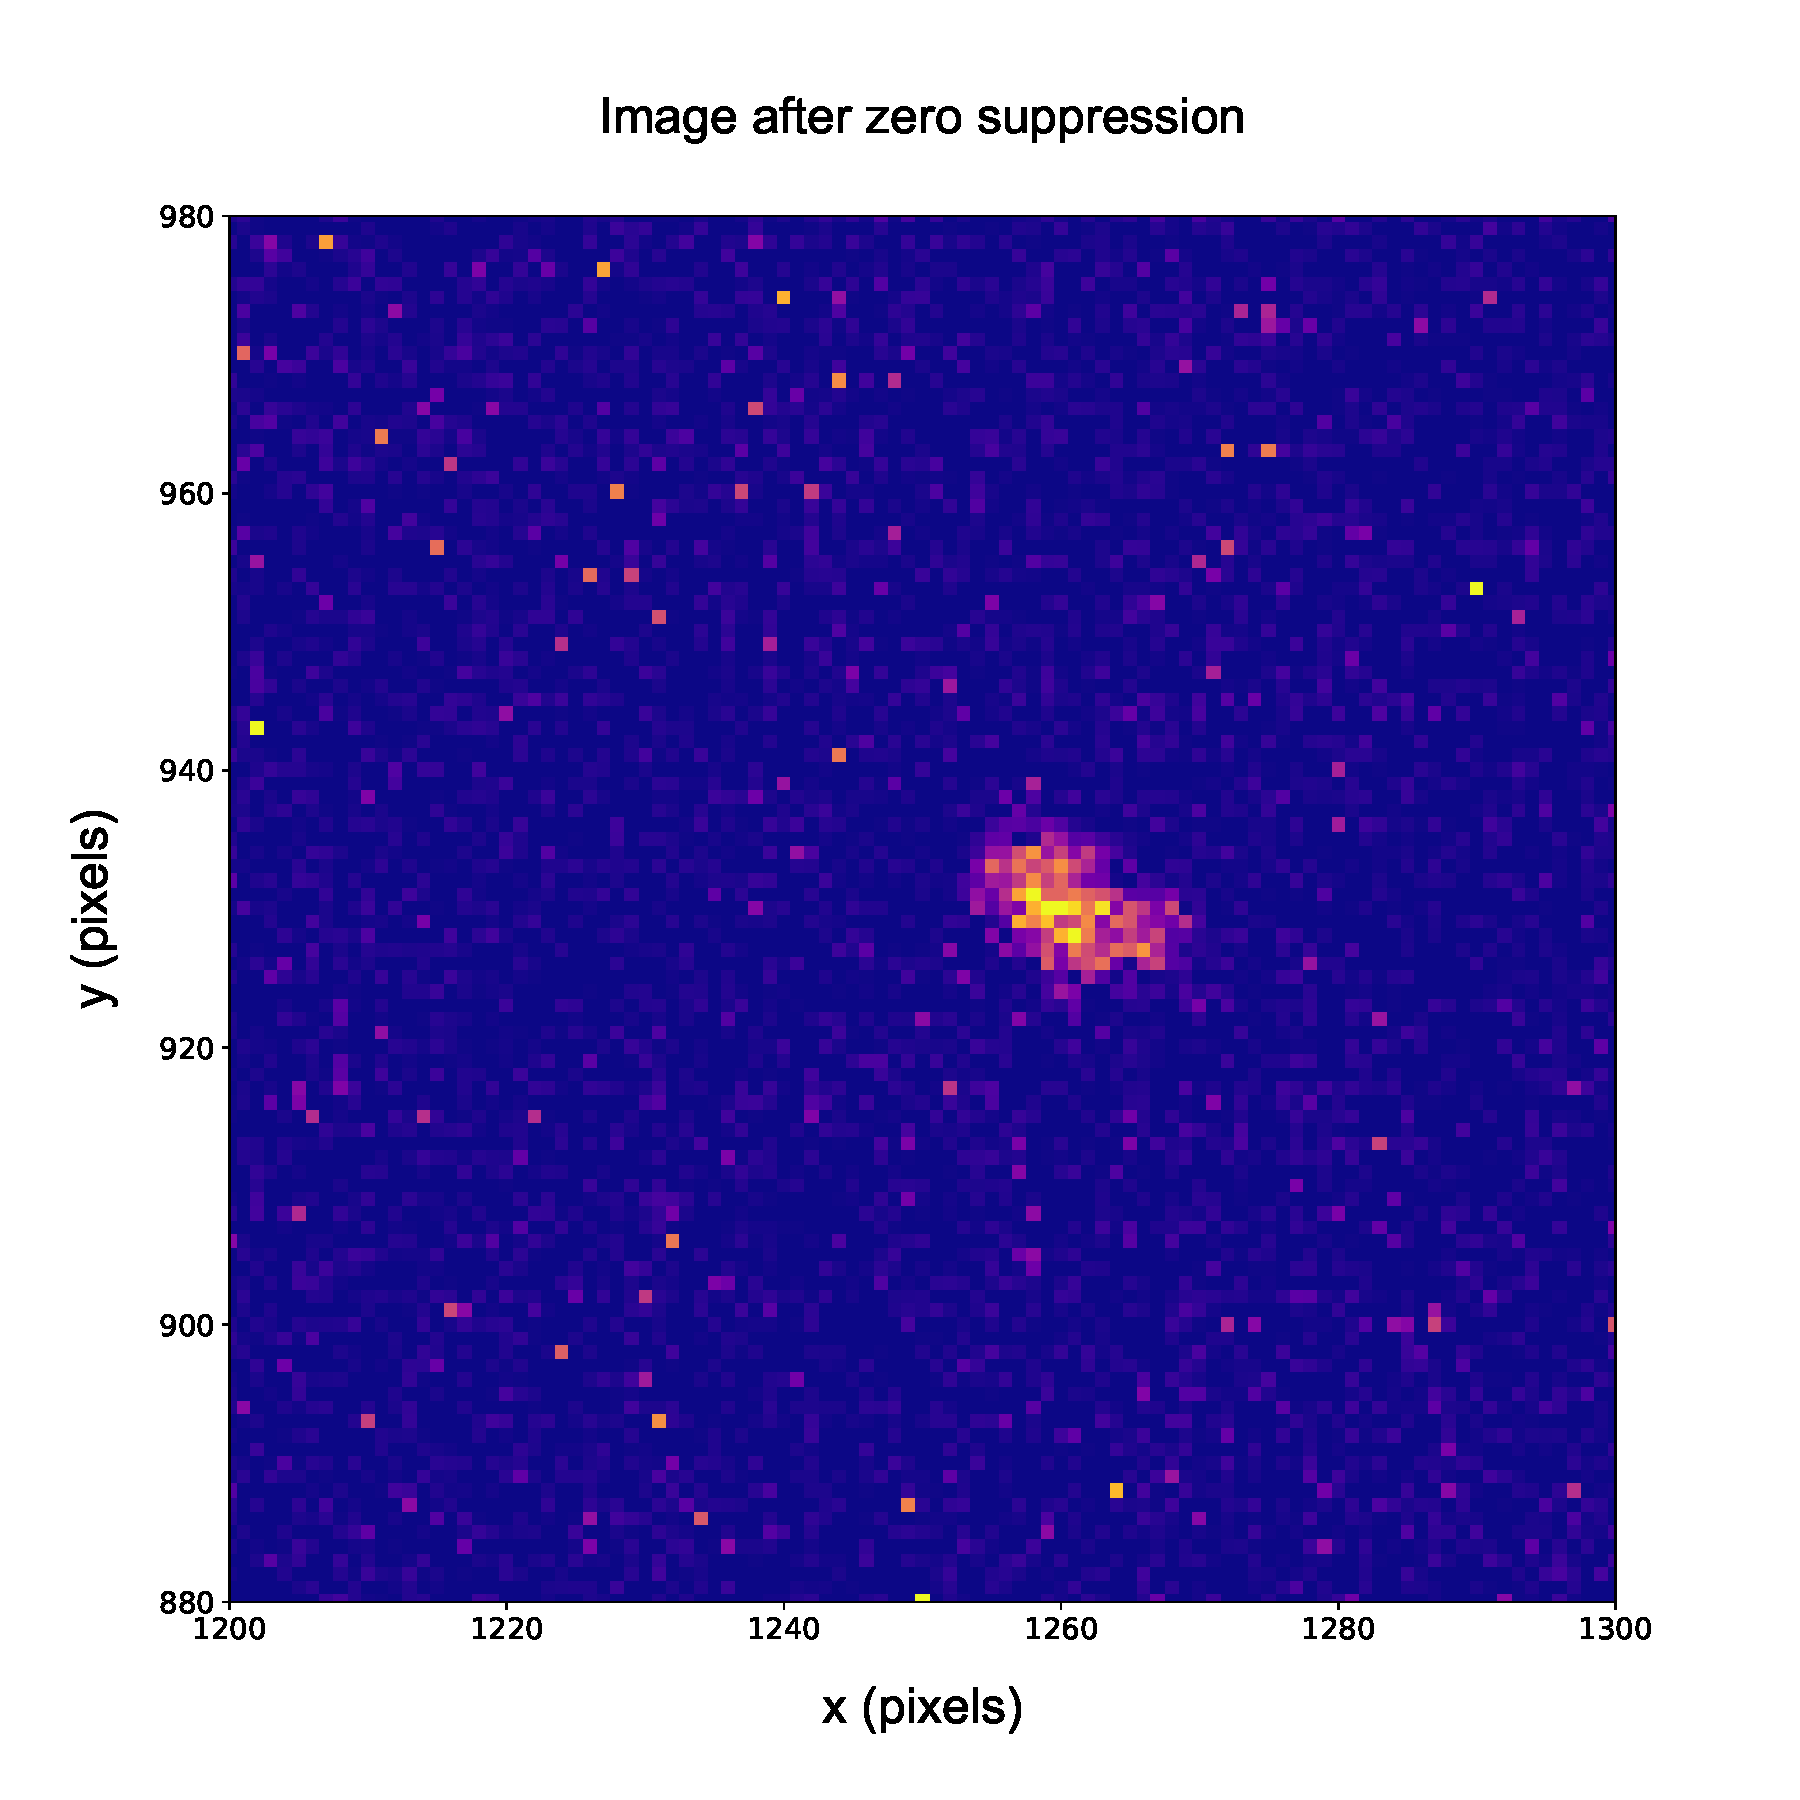
\includegraphics[width=0.49\linewidth]{figures/pic_run02097_ev317_oriIma_paper}

  \caption{Examples of two nuclear recoil candidates, selected with  the full selection, shown in a portion of $100\times100$ pixel matrix, after the zero suppression of the image. Left: a candidate
    with $E=5.2\keV$ and $\delta=10.5$, right: a candidate with
    $E=6.0\keV$ and $\delta=10$.  \label{fig:lowEnergyNR}}

\end{center}
\end{figure}

